\documentclass[1p]{elsarticle_modified}
%\bibliographystyle{elsarticle-num}

%\usepackage[colorlinks]{hyperref}
%\usepackage{abbrmath_seonhwa} %\Abb, \Ascr, \Acal ,\Abf, \Afrak
\usepackage{amsfonts}
\usepackage{amssymb}
\usepackage{amsmath}
\usepackage{amsthm}
\usepackage{scalefnt}
\usepackage{amsbsy}
\usepackage{kotex}
\usepackage{caption}
\usepackage{subfig}
\usepackage{color}
\usepackage{graphicx}
\usepackage{xcolor} %% white, black, red, green, blue, cyan, magenta, yellow
\usepackage{float}
\usepackage{setspace}
\usepackage{hyperref}

\usepackage{tikz}
\usetikzlibrary{arrows}

\usepackage{multirow}
\usepackage{array} % fixed length table
\usepackage{hhline}

%%%%%%%%%%%%%%%%%%%%%
\makeatletter
\renewcommand*\env@matrix[1][\arraystretch]{%
	\edef\arraystretch{#1}%
	\hskip -\arraycolsep
	\let\@ifnextchar\new@ifnextchar
	\array{*\c@MaxMatrixCols c}}
\makeatother %https://tex.stackexchange.com/questions/14071/how-can-i-increase-the-line-spacing-in-a-matrix
%%%%%%%%%%%%%%%

\usepackage[normalem]{ulem}

\newcommand{\msout}[1]{\ifmmode\text{\sout{\ensuremath{#1}}}\else\sout{#1}\fi}
%SOURCE: \msout is \stkout macro in https://tex.stackexchange.com/questions/20609/strikeout-in-math-mode

\newcommand{\cancel}[1]{
	\ifmmode
	{\color{red}\msout{#1}}
	\else
	{\color{red}\sout{#1}}
	\fi
}

\newcommand{\add}[1]{
	{\color{blue}\uwave{#1}}
}

\newcommand{\replace}[2]{
	\ifmmode
	{\color{red}\msout{#1}}{\color{blue}\uwave{#2}}
	\else
	{\color{red}\sout{#1}}{\color{blue}\uwave{#2}}
	\fi
}

\newcommand{\Sol}{\mathcal{S}} %segment
\newcommand{\D}{D} %diagram
\newcommand{\A}{\mathcal{A}} %arc


%%%%%%%%%%%%%%%%%%%%%%%%%%%%%5 test

\def\sl{\operatorname{\textup{SL}}(2,\Cbb)}
\def\psl{\operatorname{\textup{PSL}}(2,\Cbb)}
\def\quan{\mkern 1mu \triangleright \mkern 1mu}

\theoremstyle{definition}
\newtheorem{thm}{Theorem}[section]
\newtheorem{prop}[thm]{Proposition}
\newtheorem{lem}[thm]{Lemma}
\newtheorem{ques}[thm]{Question}
\newtheorem{cor}[thm]{Corollary}
\newtheorem{defn}[thm]{Definition}
\newtheorem{exam}[thm]{Example}
\newtheorem{rmk}[thm]{Remark}
\newtheorem{alg}[thm]{Algorithm}

\newcommand{\I}{\sqrt{-1}}
\begin{document}

%\begin{frontmatter}
%
%\title{Boundary parabolic representations of knots up to 8 crossings}
%
%%% Group authors per affiliation:
%\author{Yunhi Cho} 
%\address{Department of Mathematics, University of Seoul, Seoul, Korea}
%\ead{yhcho@uos.ac.kr}
%
%
%\author{Seonhwa Kim} %\fnref{s_kim}}
%\address{Center for Geometry and Physics, Institute for Basic Science, Pohang, 37673, Korea}
%\ead{ryeona17@ibs.re.kr}
%
%\author{Hyuk Kim}
%\address{Department of Mathematical Sciences, Seoul National University, Seoul 08826, Korea}
%\ead{hyukkim@snu.ac.kr}
%
%\author{Seokbeom Yoon}
%\address{Department of Mathematical Sciences, Seoul National University, Seoul, 08826,  Korea}
%\ead{sbyoon15@snu.ac.kr}
%
%\begin{abstract}
%We find all boundary parabolic representation of knots up to 8 crossings.
%
%\end{abstract}
%\begin{keyword}
%    \MSC[2010] 57M25 
%\end{keyword}
%
%\end{frontmatter}

%\linenumbers
%\tableofcontents
%
\newcommand\colored[1]{\textcolor{white}{\rule[-0.35ex]{0.8em}{1.4ex}}\kern-0.8em\color{red} #1}%
%\newcommand\colored[1]{\textcolor{white}{ #1}\kern-2.17ex	\textcolor{white}{ #1}\kern-1.81ex	\textcolor{white}{ #1}\kern-2.15ex\color{red}#1	}

{\Large $\underline{12a_{0456}~(K12a_{0456})}$}

\setlength{\tabcolsep}{10pt}
\renewcommand{\arraystretch}{1.6}
\vspace{1cm}\begin{tabular}{m{100pt}>{\centering\arraybackslash}m{274pt}}
\multirow{5}{120pt}{
	\centering
	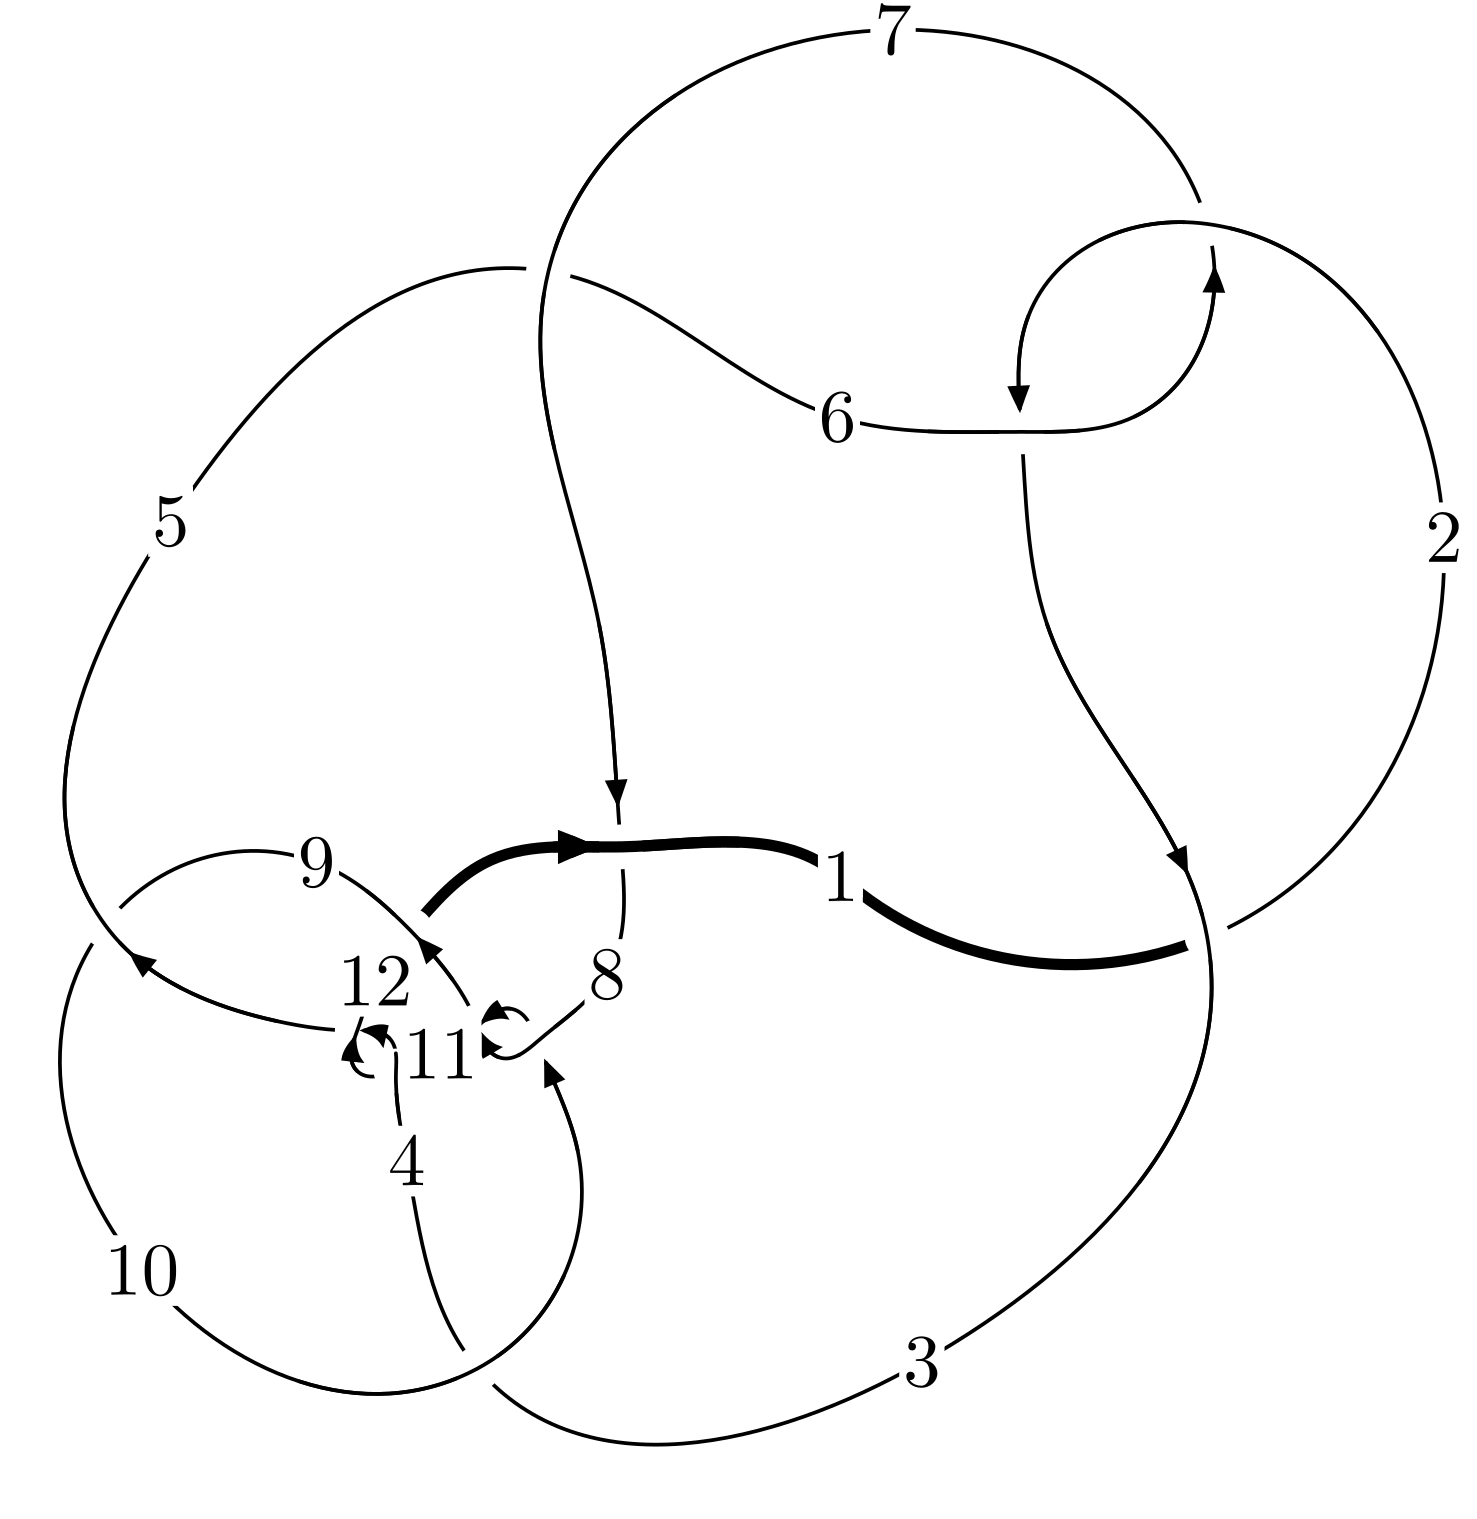
\includegraphics[width=112pt]{../../../GIT/diagram.site/Diagrams/png/1257_12a_0456.png}\\
\ \ \ A knot diagram\footnotemark}&
\allowdisplaybreaks
\textbf{Linearized knot diagam} \\
\cline{2-2}
 &
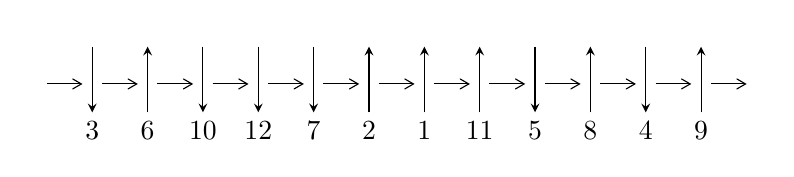
\begin{tikzpicture}[x=20pt, y=17pt]
	% nodes
	\node (C0) at (0, 0) {};
	\node (C1) at (1, 0) {};
	\node (C1U) at (1, +1) {};
	\node (C1D) at (1, -1) {3};

	\node (C2) at (2, 0) {};
	\node (C2U) at (2, +1) {};
	\node (C2D) at (2, -1) {6};

	\node (C3) at (3, 0) {};
	\node (C3U) at (3, +1) {};
	\node (C3D) at (3, -1) {10};

	\node (C4) at (4, 0) {};
	\node (C4U) at (4, +1) {};
	\node (C4D) at (4, -1) {12};

	\node (C5) at (5, 0) {};
	\node (C5U) at (5, +1) {};
	\node (C5D) at (5, -1) {7};

	\node (C6) at (6, 0) {};
	\node (C6U) at (6, +1) {};
	\node (C6D) at (6, -1) {2};

	\node (C7) at (7, 0) {};
	\node (C7U) at (7, +1) {};
	\node (C7D) at (7, -1) {1};

	\node (C8) at (8, 0) {};
	\node (C8U) at (8, +1) {};
	\node (C8D) at (8, -1) {11};

	\node (C9) at (9, 0) {};
	\node (C9U) at (9, +1) {};
	\node (C9D) at (9, -1) {5};

	\node (C10) at (10, 0) {};
	\node (C10U) at (10, +1) {};
	\node (C10D) at (10, -1) {8};

	\node (C11) at (11, 0) {};
	\node (C11U) at (11, +1) {};
	\node (C11D) at (11, -1) {4};

	\node (C12) at (12, 0) {};
	\node (C12U) at (12, +1) {};
	\node (C12D) at (12, -1) {9};
	\node (C13) at (13, 0) {};

	% arrows
	\draw[->,>={angle 60}]
	(C0) edge (C1) (C1) edge (C2) (C2) edge (C3) (C3) edge (C4) (C4) edge (C5) (C5) edge (C6) (C6) edge (C7) (C7) edge (C8) (C8) edge (C9) (C9) edge (C10) (C10) edge (C11) (C11) edge (C12) (C12) edge (C13) ;	\draw[->,>=stealth]
	(C1U) edge (C1D) (C2D) edge (C2U) (C3U) edge (C3D) (C4U) edge (C4D) (C5U) edge (C5D) (C6D) edge (C6U) (C7D) edge (C7U) (C8D) edge (C8U) (C9U) edge (C9D) (C10D) edge (C10U) (C11U) edge (C11D) (C12D) edge (C12U) ;
	\end{tikzpicture} \\
\hhline{~~} \\& 
\textbf{Solving Sequence} \\ \cline{2-2} 
 &
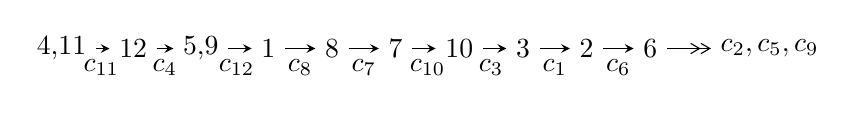
\begin{tikzpicture}[x=23pt, y=7pt]
	% node
	\node (A0) at (-1/8, 0) {4,11};
	\node (A1) at (1, 0) {12};
	\node (A2) at (33/16, 0) {5,9};
	\node (A3) at (25/8, 0) {1};
	\node (A4) at (33/8, 0) {8};
	\node (A5) at (41/8, 0) {7};
	\node (A6) at (49/8, 0) {10};
	\node (A7) at (57/8, 0) {3};
	\node (A8) at (65/8, 0) {2};
	\node (A9) at (73/8, 0) {6};
	\node (C1) at (1/2, -1) {$c_{11}$};
	\node (C2) at (3/2, -1) {$c_{4}$};
	\node (C3) at (21/8, -1) {$c_{12}$};
	\node (C4) at (29/8, -1) {$c_{8}$};
	\node (C5) at (37/8, -1) {$c_{7}$};
	\node (C6) at (45/8, -1) {$c_{10}$};
	\node (C7) at (53/8, -1) {$c_{3}$};
	\node (C8) at (61/8, -1) {$c_{1}$};
	\node (C9) at (69/8, -1) {$c_{6}$};
	\node (A10) at (11, 0) {$c_{2},c_{5},c_{9}$};

	% edge
	\draw[->,>=stealth]	
	(A0) edge (A1) (A1) edge (A2) (A2) edge (A3) (A3) edge (A4) (A4) edge (A5) (A5) edge (A6) (A6) edge (A7) (A7) edge (A8) (A8) edge (A9) ;
	\draw[->>,>={angle 60}]	
	(A9) edge (A10);
\end{tikzpicture} \\ 

\end{tabular} \\

\footnotetext{
The image of knot diagram is generated by the software ``\textbf{Draw programme}" developed by Andrew Bartholomew(\url{http://www.layer8.co.uk/maths/draw/index.htm\#Running-draw}), where we modified some parts for our purpose(\url{https://github.com/CATsTAILs/LinksPainter}).
}\phantom \\ \newline 
\centering \textbf{Ideals for irreducible components\footnotemark of $X_{\text{par}}$} 
 
\begin{align*}
I^u_{1}&=\langle 
-2.53175\times10^{313} u^{115}+2.92436\times10^{313} u^{114}+\cdots+2.25234\times10^{314} b+8.23829\times10^{313},\\
\phantom{I^u_{1}}&\phantom{= \langle  }-2.24989\times10^{314} u^{115}+2.20110\times10^{314} u^{114}+\cdots+3.60375\times10^{315} a-2.99578\times10^{315},\\
\phantom{I^u_{1}}&\phantom{= \langle  }u^{116}+2 u^{115}+\cdots+4 u+1\rangle \\
I^u_{2}&=\langle 
b-1,\;3 u^3+2 u^2+16 a+7 u+11,\;u^4- u^3+3 u^2-2 u+1\rangle \\
\\
\end{align*}
\raggedright * 2 irreducible components of $\dim_{\mathbb{C}}=0$, with total 120 representations.\\
\footnotetext{All coefficients of polynomials are rational numbers. But the coefficients are sometimes approximated in decimal forms when there is not enough margin.}
\newpage
\renewcommand{\arraystretch}{1}
\centering \section*{I. $I^u_{1}= \langle -2.53\times10^{313} u^{115}+2.92\times10^{313} u^{114}+\cdots+2.25\times10^{314} b+8.24\times10^{313},\;-2.25\times10^{314} u^{115}+2.20\times10^{314} u^{114}+\cdots+3.60\times10^{315} a-3.00\times10^{315},\;u^{116}+2 u^{115}+\cdots+4 u+1 \rangle$}
\flushleft \textbf{(i) Arc colorings}\\
\begin{tabular}{m{7pt} m{180pt} m{7pt} m{180pt} }
\flushright $a_{4}=$&$\begin{pmatrix}0\\u\end{pmatrix}$ \\
\flushright $a_{11}=$&$\begin{pmatrix}1\\0\end{pmatrix}$ \\
\flushright $a_{12}=$&$\begin{pmatrix}1\\u^2\end{pmatrix}$ \\
\flushright $a_{5}=$&$\begin{pmatrix}- u\\- u^3+u\end{pmatrix}$ \\
\flushright $a_{9}=$&$\begin{pmatrix}0.0624320 u^{115}-0.0610780 u^{114}+\cdots-0.624844 u+0.831296\\0.112405 u^{115}-0.129836 u^{114}+\cdots-3.13673 u-0.365765\end{pmatrix}$ \\
\flushright $a_{1}=$&$\begin{pmatrix}-1.36566 u^{115}-0.966684 u^{114}+\cdots-0.101173 u+0.236304\\-0.0575097 u^{115}+0.109899 u^{114}+\cdots+3.11321 u+0.437787\end{pmatrix}$ \\
\flushright $a_{8}=$&$\begin{pmatrix}-0.0499731 u^{115}+0.0687581 u^{114}+\cdots+2.51188 u+1.19706\\0.112405 u^{115}-0.129836 u^{114}+\cdots-3.13673 u-0.365765\end{pmatrix}$ \\
\flushright $a_{7}=$&$\begin{pmatrix}0.376542 u^{115}+0.0535687 u^{114}+\cdots+0.455051 u+0.877028\\-0.313567 u^{115}-1.13025 u^{114}+\cdots-9.22734 u-2.08951\end{pmatrix}$ \\
\flushright $a_{10}=$&$\begin{pmatrix}-0.0577405 u^{115}-0.359290 u^{114}+\cdots-2.23769 u+0.421032\\0.277384 u^{115}+0.258423 u^{114}+\cdots-1.17224 u+0.102366\end{pmatrix}$ \\
\flushright $a_{3}=$&$\begin{pmatrix}1.10683 u^{115}+1.22497 u^{114}+\cdots+5.46904 u+1.96029\\-0.608411 u^{115}-1.03975 u^{114}+\cdots-1.36203 u-0.474932\end{pmatrix}$ \\
\flushright $a_{2}=$&$\begin{pmatrix}-0.448108 u^{115}+1.00733 u^{114}+\cdots+7.64578 u+1.31221\\0.191247 u^{115}+0.929848 u^{114}+\cdots+9.34460 u+2.37131\end{pmatrix}$ \\
\flushright $a_{6}=$&$\begin{pmatrix}0.269740 u^{115}+0.274312 u^{114}+\cdots-2.62641 u-1.27309\\2.08463 u^{115}+3.62773 u^{114}+\cdots+8.91773 u+0.133485\end{pmatrix}$\\&\end{tabular}
\flushleft \textbf{(ii) Obstruction class $= -1$}\\~\\
\flushleft \textbf{(iii) Cusp Shapes $= -4.00070 u^{115}-9.56340 u^{114}+\cdots-41.1381 u-13.7651$}\\~\\
\newpage\renewcommand{\arraystretch}{1}
\flushleft \textbf{(iv) u-Polynomials at the component}\newline \\
\begin{tabular}{m{50pt}|m{274pt}}
Crossings & \hspace{64pt}u-Polynomials at each crossing \\
\hline $$\begin{aligned}c_{1},c_{5}\end{aligned}$$&$\begin{aligned}
&u^{116}+38 u^{115}+\cdots-2 u+1
\end{aligned}$\\
\hline $$\begin{aligned}c_{2},c_{6}\end{aligned}$$&$\begin{aligned}
&u^{116}-2 u^{115}+\cdots- u^2+1
\end{aligned}$\\
\hline $$\begin{aligned}c_{3}\end{aligned}$$&$\begin{aligned}
&16(16 u^{116}-117 u^{115}+\cdots-5135 u+3001)
\end{aligned}$\\
\hline $$\begin{aligned}c_{4},c_{11}\end{aligned}$$&$\begin{aligned}
&u^{116}+2 u^{115}+\cdots+4 u+1
\end{aligned}$\\
\hline $$\begin{aligned}c_{7}\end{aligned}$$&$\begin{aligned}
&u^{116}+10 u^{115}+\cdots+1233680 u+97600
\end{aligned}$\\
\hline $$\begin{aligned}c_{8},c_{10}\end{aligned}$$&$\begin{aligned}
&u^{116}+5 u^{115}+\cdots+2505 u+256
\end{aligned}$\\
\hline $$\begin{aligned}c_{9}\end{aligned}$$&$\begin{aligned}
&u^{116}+3 u^{115}+\cdots+26496 u+4096
\end{aligned}$\\
\hline $$\begin{aligned}c_{12}\end{aligned}$$&$\begin{aligned}
&16(16 u^{116}+237 u^{115}+\cdots-7715 u+289)
\end{aligned}$\\
\hline
\end{tabular}\\~\\
\newpage\renewcommand{\arraystretch}{1}
\flushleft \textbf{(v) Riley Polynomials at the component}\newline \\
\begin{tabular}{m{50pt}|m{274pt}}
Crossings & \hspace{64pt}Riley Polynomials at each crossing \\
\hline $$\begin{aligned}c_{1},c_{5}\end{aligned}$$&$\begin{aligned}
&y^{116}+82 y^{115}+\cdots-14 y+1
\end{aligned}$\\
\hline $$\begin{aligned}c_{2},c_{6}\end{aligned}$$&$\begin{aligned}
&y^{116}+38 y^{115}+\cdots-2 y+1
\end{aligned}$\\
\hline $$\begin{aligned}c_{3}\end{aligned}$$&$\begin{aligned}
&256(256 y^{116}+3815 y^{115}+\cdots-5.95490\times10^{8} y+9006001)
\end{aligned}$\\
\hline $$\begin{aligned}c_{4},c_{11}\end{aligned}$$&$\begin{aligned}
&y^{116}-62 y^{115}+\cdots-2 y+1
\end{aligned}$\\
\hline $$\begin{aligned}c_{7}\end{aligned}$$&$\begin{aligned}
&y^{116}+14 y^{115}+\cdots+306040470400 y+9525760000
\end{aligned}$\\
\hline $$\begin{aligned}c_{8},c_{10}\end{aligned}$$&$\begin{aligned}
&y^{116}-67 y^{115}+\cdots-938449 y+65536
\end{aligned}$\\
\hline $$\begin{aligned}c_{9}\end{aligned}$$&$\begin{aligned}
&y^{116}-27 y^{115}+\cdots+438878208 y+16777216
\end{aligned}$\\
\hline $$\begin{aligned}c_{12}\end{aligned}$$&$\begin{aligned}
&256(256 y^{116}+14007 y^{115}+\cdots-1.71712\times10^{7} y+83521)
\end{aligned}$\\
\hline
\end{tabular}\\~\\
\newpage\flushleft \textbf{(vi) Complex Volumes and Cusp Shapes}
$$\begin{array}{c|c|c}  
\text{Solutions to }I^u_{1}& \I (\text{vol} + \sqrt{-1}CS) & \text{Cusp shape}\\
 \hline 
\begin{aligned}
u &= \phantom{-}0.932975 + 0.380055 I \\
a &= \phantom{-}0.50615 - 1.93295 I \\
b &= \phantom{-}1.18511 - 0.91051 I\end{aligned}
 & \phantom{-}3.59446 - 4.25759 I & \phantom{-0.000000 } 0 \\ \hline\begin{aligned}
u &= \phantom{-}0.932975 - 0.380055 I \\
a &= \phantom{-}0.50615 + 1.93295 I \\
b &= \phantom{-}1.18511 + 0.91051 I\end{aligned}
 & \phantom{-}3.59446 + 4.25759 I & \phantom{-0.000000 } 0 \\ \hline\begin{aligned}
u &= -0.942443 + 0.386528 I \\
a &= \phantom{-}0.48712 + 1.95718 I \\
b &= \phantom{-}1.16351 + 0.96120 I\end{aligned}
 & \phantom{-}2.72521 + 9.87166 I & \phantom{-0.000000 } 0 \\ \hline\begin{aligned}
u &= -0.942443 - 0.386528 I \\
a &= \phantom{-}0.48712 - 1.95718 I \\
b &= \phantom{-}1.16351 - 0.96120 I\end{aligned}
 & \phantom{-}2.72521 - 9.87166 I & \phantom{-0.000000 } 0 \\ \hline\begin{aligned}
u &= -1.015520 + 0.079924 I \\
a &= \phantom{-}2.86594 + 5.65897 I \\
b &= \phantom{-}0.943003 - 0.008732 I\end{aligned}
 & \phantom{-}1.51330 - 0.01120 I & \phantom{-0.000000 } 0 \\ \hline\begin{aligned}
u &= -1.015520 - 0.079924 I \\
a &= \phantom{-}2.86594 - 5.65897 I \\
b &= \phantom{-}0.943003 + 0.008732 I\end{aligned}
 & \phantom{-}1.51330 + 0.01120 I & \phantom{-0.000000 } 0 \\ \hline\begin{aligned}
u &= \phantom{-}0.921677 + 0.322581 I \\
a &= \phantom{-}0.47350 - 1.83013 I \\
b &= \phantom{-}1.102010 - 0.674058 I\end{aligned}
 & \phantom{-}1.18239 - 2.90297 I & \phantom{-0.000000 } 0 \\ \hline\begin{aligned}
u &= \phantom{-}0.921677 - 0.322581 I \\
a &= \phantom{-}0.47350 + 1.83013 I \\
b &= \phantom{-}1.102010 + 0.674058 I\end{aligned}
 & \phantom{-}1.18239 + 2.90297 I & \phantom{-0.000000 } 0 \\ \hline\begin{aligned}
u &= -0.966971 + 0.356693 I \\
a &= \phantom{-}0.42098 + 1.89144 I \\
b &= \phantom{-}0.991776 + 0.891367 I\end{aligned}
 & -2.25470 + 4.58566 I & \phantom{-0.000000 } 0 \\ \hline\begin{aligned}
u &= -0.966971 - 0.356693 I \\
a &= \phantom{-}0.42098 - 1.89144 I \\
b &= \phantom{-}0.991776 - 0.891367 I\end{aligned}
 & -2.25470 - 4.58566 I & \phantom{-0.000000 } 0\\
 \hline 
 \end{array}$$\newpage$$\begin{array}{c|c|c}  
\text{Solutions to }I^u_{1}& \I (\text{vol} + \sqrt{-1}CS) & \text{Cusp shape}\\
 \hline 
\begin{aligned}
u &= \phantom{-}1.025030 + 0.133441 I \\
a &= \phantom{-}2.16050 - 2.96069 I \\
b &= \phantom{-}0.820014 - 0.004042 I\end{aligned}
 & -3.74478 - 0.00361 I & \phantom{-0.000000 } 0 \\ \hline\begin{aligned}
u &= \phantom{-}1.025030 - 0.133441 I \\
a &= \phantom{-}2.16050 + 2.96069 I \\
b &= \phantom{-}0.820014 + 0.004042 I\end{aligned}
 & -3.74478 + 0.00361 I & \phantom{-0.000000 } 0 \\ \hline\begin{aligned}
u &= \phantom{-}1.032360 + 0.089616 I \\
a &= \phantom{-}3.52581 - 4.46017 I \\
b &= \phantom{-}0.924511 + 0.036679 I\end{aligned}
 & \phantom{-}0.64084 + 5.41192 I & \phantom{-0.000000 } 0 \\ \hline\begin{aligned}
u &= \phantom{-}1.032360 - 0.089616 I \\
a &= \phantom{-}3.52581 + 4.46017 I \\
b &= \phantom{-}0.924511 - 0.036679 I\end{aligned}
 & \phantom{-}0.64084 - 5.41192 I & \phantom{-0.000000 } 0 \\ \hline\begin{aligned}
u &= -0.933101 + 0.165578 I \\
a &= \phantom{-}0.15820 + 2.41425 I \\
b &= \phantom{-}0.963208 + 0.212678 I\end{aligned}
 & \phantom{-}0.097528 + 0.717924 I & \phantom{-0.000000 } 0 \\ \hline\begin{aligned}
u &= -0.933101 - 0.165578 I \\
a &= \phantom{-}0.15820 - 2.41425 I \\
b &= \phantom{-}0.963208 - 0.212678 I\end{aligned}
 & \phantom{-}0.097528 - 0.717924 I & \phantom{-0.000000 } 0 \\ \hline\begin{aligned}
u &= \phantom{-}1.040820 + 0.176639 I \\
a &= \phantom{-}1.70112 - 1.62243 I \\
b &= \phantom{-}0.587537 - 0.040637 I\end{aligned}
 & -0.10015 - 5.28988 I & \phantom{-0.000000 } 0 \\ \hline\begin{aligned}
u &= \phantom{-}1.040820 - 0.176639 I \\
a &= \phantom{-}1.70112 + 1.62243 I \\
b &= \phantom{-}0.587537 + 0.040637 I\end{aligned}
 & -0.10015 + 5.28988 I & \phantom{-0.000000 } 0 \\ \hline\begin{aligned}
u &= -1.051100 + 0.195133 I \\
a &= \phantom{-}1.13277 + 1.30258 I \\
b &= \phantom{-}0.433420 + 0.197090 I\end{aligned}
 & \phantom{-}0.514456 + 0.135291 I & \phantom{-0.000000 } 0 \\ \hline\begin{aligned}
u &= -1.051100 - 0.195133 I \\
a &= \phantom{-}1.13277 - 1.30258 I \\
b &= \phantom{-}0.433420 - 0.197090 I\end{aligned}
 & \phantom{-}0.514456 - 0.135291 I & \phantom{-0.000000 } 0\\
 \hline 
 \end{array}$$\newpage$$\begin{array}{c|c|c}  
\text{Solutions to }I^u_{1}& \I (\text{vol} + \sqrt{-1}CS) & \text{Cusp shape}\\
 \hline 
\begin{aligned}
u &= -0.168018 + 1.071190 I \\
a &= \phantom{-}0.338703 + 0.172300 I \\
b &= -1.151900 + 0.484030 I\end{aligned}
 & -1.45169 - 6.87895 I & \phantom{-0.000000 } 0 \\ \hline\begin{aligned}
u &= -0.168018 - 1.071190 I \\
a &= \phantom{-}0.338703 - 0.172300 I \\
b &= -1.151900 - 0.484030 I\end{aligned}
 & -1.45169 + 6.87895 I & \phantom{-0.000000 } 0 \\ \hline\begin{aligned}
u &= \phantom{-}0.837697 + 0.351028 I \\
a &= \phantom{-}0.63116 - 1.69354 I \\
b &= \phantom{-}1.40819 - 0.57266 I\end{aligned}
 & \phantom{-}4.57854 - 2.68459 I & \phantom{-0.000000 } 0 \\ \hline\begin{aligned}
u &= \phantom{-}0.837697 - 0.351028 I \\
a &= \phantom{-}0.63116 + 1.69354 I \\
b &= \phantom{-}1.40819 + 0.57266 I\end{aligned}
 & \phantom{-}4.57854 + 2.68459 I & \phantom{-0.000000 } 0 \\ \hline\begin{aligned}
u &= -0.133686 + 1.084940 I \\
a &= \phantom{-}0.288829 + 0.186794 I \\
b &= -1.250560 + 0.482907 I\end{aligned}
 & \phantom{-}4.19362 - 13.02090 I & \phantom{-0.000000 } 0 \\ \hline\begin{aligned}
u &= -0.133686 - 1.084940 I \\
a &= \phantom{-}0.288829 - 0.186794 I \\
b &= -1.250560 - 0.482907 I\end{aligned}
 & \phantom{-}4.19362 + 13.02090 I & \phantom{-0.000000 } 0 \\ \hline\begin{aligned}
u &= -0.255673 + 1.064880 I \\
a &= \phantom{-}0.403088 + 0.100874 I \\
b &= -1.002170 + 0.401779 I\end{aligned}
 & \phantom{-}0.405726 - 0.191311 I & \phantom{-0.000000 } 0 \\ \hline\begin{aligned}
u &= -0.255673 - 1.064880 I \\
a &= \phantom{-}0.403088 - 0.100874 I \\
b &= -1.002170 - 0.401779 I\end{aligned}
 & \phantom{-}0.405726 + 0.191311 I & \phantom{-0.000000 } 0 \\ \hline\begin{aligned}
u &= \phantom{-}0.139068 + 1.094320 I \\
a &= \phantom{-}0.288556 - 0.170981 I \\
b &= -1.242370 - 0.453261 I\end{aligned}
 & \phantom{-}5.30484 + 7.16529 I & \phantom{-0.000000 } 0 \\ \hline\begin{aligned}
u &= \phantom{-}0.139068 - 1.094320 I \\
a &= \phantom{-}0.288556 + 0.170981 I \\
b &= -1.242370 + 0.453261 I\end{aligned}
 & \phantom{-}5.30484 - 7.16529 I & \phantom{-0.000000 } 0\\
 \hline 
 \end{array}$$\newpage$$\begin{array}{c|c|c}  
\text{Solutions to }I^u_{1}& \I (\text{vol} + \sqrt{-1}CS) & \text{Cusp shape}\\
 \hline 
\begin{aligned}
u &= -1.064290 + 0.320997 I \\
a &= \phantom{-}0.25708 + 1.62401 I \\
b &= \phantom{-}0.484658 + 0.861383 I\end{aligned}
 & \phantom{-}0.553410 - 0.120359 I & \phantom{-0.000000 } 0 \\ \hline\begin{aligned}
u &= -1.064290 - 0.320997 I \\
a &= \phantom{-}0.25708 - 1.62401 I \\
b &= \phantom{-}0.484658 - 0.861383 I\end{aligned}
 & \phantom{-}0.553410 + 0.120359 I & \phantom{-0.000000 } 0 \\ \hline\begin{aligned}
u &= -0.815607 + 0.351086 I \\
a &= \phantom{-}0.66682 + 1.62768 I \\
b &= \phantom{-}1.45666 + 0.51569 I\end{aligned}
 & \phantom{-}4.00667 - 2.83899 I & \phantom{-0.000000 } 0 \\ \hline\begin{aligned}
u &= -0.815607 - 0.351086 I \\
a &= \phantom{-}0.66682 - 1.62768 I \\
b &= \phantom{-}1.45666 - 0.51569 I\end{aligned}
 & \phantom{-}4.00667 + 2.83899 I & \phantom{-0.000000 } 0 \\ \hline\begin{aligned}
u &= \phantom{-}0.197323 + 1.109430 I \\
a &= \phantom{-}0.334392 - 0.117534 I \\
b &= -1.125740 - 0.385168 I\end{aligned}
 & \phantom{-}2.84490 + 4.28893 I & \phantom{-0.000000 } 0 \\ \hline\begin{aligned}
u &= \phantom{-}0.197323 - 1.109430 I \\
a &= \phantom{-}0.334392 + 0.117534 I \\
b &= -1.125740 + 0.385168 I\end{aligned}
 & \phantom{-}2.84490 - 4.28893 I & \phantom{-0.000000 } 0 \\ \hline\begin{aligned}
u &= \phantom{-}1.108580 + 0.330328 I \\
a &= \phantom{-}0.07789 - 1.50159 I \\
b &= \phantom{-}0.268886 - 0.939607 I\end{aligned}
 & \phantom{-}0.73853 - 5.21162 I & \phantom{-0.000000 } 0 \\ \hline\begin{aligned}
u &= \phantom{-}1.108580 - 0.330328 I \\
a &= \phantom{-}0.07789 + 1.50159 I \\
b &= \phantom{-}0.268886 + 0.939607 I\end{aligned}
 & \phantom{-}0.73853 + 5.21162 I & \phantom{-0.000000 } 0 \\ \hline\begin{aligned}
u &= \phantom{-}1.030480 + 0.600228 I \\
a &= \phantom{-}0.787511 + 0.802602 I \\
b &= -0.629673 + 0.394217 I\end{aligned}
 & -1.91929 + 4.20741 I & \phantom{-0.000000 } 0 \\ \hline\begin{aligned}
u &= \phantom{-}1.030480 - 0.600228 I \\
a &= \phantom{-}0.787511 - 0.802602 I \\
b &= -0.629673 - 0.394217 I\end{aligned}
 & -1.91929 - 4.20741 I & \phantom{-0.000000 } 0\\
 \hline 
 \end{array}$$\newpage$$\begin{array}{c|c|c}  
\text{Solutions to }I^u_{1}& \I (\text{vol} + \sqrt{-1}CS) & \text{Cusp shape}\\
 \hline 
\begin{aligned}
u &= -1.033930 + 0.672720 I \\
a &= \phantom{-}0.632515 - 0.738424 I \\
b &= -0.713327 - 0.320995 I\end{aligned}
 & -0.60389 + 1.31728 I & \phantom{-0.000000 } 0 \\ \hline\begin{aligned}
u &= -1.033930 - 0.672720 I \\
a &= \phantom{-}0.632515 + 0.738424 I \\
b &= -0.713327 + 0.320995 I\end{aligned}
 & -0.60389 - 1.31728 I & \phantom{-0.000000 } 0 \\ \hline\begin{aligned}
u &= -0.712038 + 0.268205 I \\
a &= \phantom{-}0.544099 + 1.124880 I \\
b &= \phantom{-}1.41778 + 0.18424 I\end{aligned}
 & -0.13211 + 1.45451 I & -1.69686 - 4.01852 I \\ \hline\begin{aligned}
u &= -0.712038 - 0.268205 I \\
a &= \phantom{-}0.544099 - 1.124880 I \\
b &= \phantom{-}1.41778 - 0.18424 I\end{aligned}
 & -0.13211 - 1.45451 I & -1.69686 + 4.01852 I \\ \hline\begin{aligned}
u &= \phantom{-}0.239199 + 0.710424 I \\
a &= \phantom{-}0.779803 - 0.124579 I \\
b &= -0.398169 - 0.538145 I\end{aligned}
 & -1.17035 + 3.60756 I & -3.17763 - 3.80286 I \\ \hline\begin{aligned}
u &= \phantom{-}0.239199 - 0.710424 I \\
a &= \phantom{-}0.779803 + 0.124579 I \\
b &= -0.398169 + 0.538145 I\end{aligned}
 & -1.17035 - 3.60756 I & -3.17763 + 3.80286 I \\ \hline\begin{aligned}
u &= \phantom{-}1.190100 + 0.393431 I \\
a &= -0.50179 - 1.42134 I \\
b &= -0.195049 - 1.264670 I\end{aligned}
 & -1.98641 - 6.48143 I & \phantom{-0.000000 } 0 \\ \hline\begin{aligned}
u &= \phantom{-}1.190100 - 0.393431 I \\
a &= -0.50179 + 1.42134 I \\
b &= -0.195049 + 1.264670 I\end{aligned}
 & -1.98641 + 6.48143 I & \phantom{-0.000000 } 0 \\ \hline\begin{aligned}
u &= \phantom{-}1.205200 + 0.360020 I \\
a &= -0.401169 - 1.223780 I \\
b &= -0.236390 - 1.062780 I\end{aligned}
 & -3.83829 - 4.36811 I & \phantom{-0.000000 } 0 \\ \hline\begin{aligned}
u &= \phantom{-}1.205200 - 0.360020 I \\
a &= -0.401169 + 1.223780 I \\
b &= -0.236390 + 1.062780 I\end{aligned}
 & -3.83829 + 4.36811 I & \phantom{-0.000000 } 0\\
 \hline 
 \end{array}$$\newpage$$\begin{array}{c|c|c}  
\text{Solutions to }I^u_{1}& \I (\text{vol} + \sqrt{-1}CS) & \text{Cusp shape}\\
 \hline 
\begin{aligned}
u &= -1.193840 + 0.399946 I \\
a &= -0.54952 + 1.42991 I \\
b &= -0.225922 + 1.298760 I\end{aligned}
 & -3.05221 + 12.12590 I & \phantom{-0.000000 } 0 \\ \hline\begin{aligned}
u &= -1.193840 - 0.399946 I \\
a &= -0.54952 - 1.42991 I \\
b &= -0.225922 - 1.298760 I\end{aligned}
 & -3.05221 - 12.12590 I & \phantom{-0.000000 } 0 \\ \hline\begin{aligned}
u &= -1.211410 + 0.388213 I \\
a &= -0.559229 + 1.294670 I \\
b &= -0.310138 + 1.203680 I\end{aligned}
 & -8.10394 + 6.21848 I & \phantom{-0.000000 } 0 \\ \hline\begin{aligned}
u &= -1.211410 - 0.388213 I \\
a &= -0.559229 - 1.294670 I \\
b &= -0.310138 - 1.203680 I\end{aligned}
 & -8.10394 - 6.21848 I & \phantom{-0.000000 } 0 \\ \hline\begin{aligned}
u &= \phantom{-}1.133830 + 0.616400 I \\
a &= \phantom{-}0.594258 + 1.041120 I \\
b &= -0.797894 + 0.496771 I\end{aligned}
 & -6.67592 - 2.20639 I & \phantom{-0.000000 } 0 \\ \hline\begin{aligned}
u &= \phantom{-}1.133830 - 0.616400 I \\
a &= \phantom{-}0.594258 - 1.041120 I \\
b &= -0.797894 - 0.496771 I\end{aligned}
 & -6.67592 + 2.20639 I & \phantom{-0.000000 } 0 \\ \hline\begin{aligned}
u &= -1.238500 + 0.366883 I \\
a &= -0.541186 + 1.087490 I \\
b &= -0.411510 + 1.043980 I\end{aligned}
 & -5.39668 + 0.15552 I & \phantom{-0.000000 } 0 \\ \hline\begin{aligned}
u &= -1.238500 - 0.366883 I \\
a &= -0.541186 - 1.087490 I \\
b &= -0.411510 - 1.043980 I\end{aligned}
 & -5.39668 - 0.15552 I & \phantom{-0.000000 } 0 \\ \hline\begin{aligned}
u &= -0.619178 + 0.338799 I \\
a &= \phantom{-}0.942625 + 0.930733 I \\
b &= \phantom{-}1.57822 + 0.02039 I\end{aligned}
 & \phantom{-}4.51489 + 6.13738 I & \phantom{-}5.17778 - 7.54514 I \\ \hline\begin{aligned}
u &= -0.619178 - 0.338799 I \\
a &= \phantom{-}0.942625 - 0.930733 I \\
b &= \phantom{-}1.57822 - 0.02039 I\end{aligned}
 & \phantom{-}4.51489 - 6.13738 I & \phantom{-}5.17778 + 7.54514 I\\
 \hline 
 \end{array}$$\newpage$$\begin{array}{c|c|c}  
\text{Solutions to }I^u_{1}& \I (\text{vol} + \sqrt{-1}CS) & \text{Cusp shape}\\
 \hline 
\begin{aligned}
u &= \phantom{-}0.593224 + 0.328294 I \\
a &= \phantom{-}0.945133 - 0.834395 I \\
b &= \phantom{-}1.54650 + 0.02847 I\end{aligned}
 & \phantom{-}5.21239 - 0.58460 I & \phantom{-}6.91499 + 2.03694 I \\ \hline\begin{aligned}
u &= \phantom{-}0.593224 - 0.328294 I \\
a &= \phantom{-}0.945133 + 0.834395 I \\
b &= \phantom{-}1.54650 - 0.02847 I\end{aligned}
 & \phantom{-}5.21239 + 0.58460 I & \phantom{-}6.91499 - 2.03694 I \\ \hline\begin{aligned}
u &= \phantom{-}1.287070 + 0.320286 I \\
a &= -0.445671 - 0.757330 I \\
b &= -0.517943 - 0.762187 I\end{aligned}
 & -4.95775 - 3.95723 I & \phantom{-0.000000 } 0 \\ \hline\begin{aligned}
u &= \phantom{-}1.287070 - 0.320286 I \\
a &= -0.445671 + 0.757330 I \\
b &= -0.517943 + 0.762187 I\end{aligned}
 & -4.95775 + 3.95723 I & \phantom{-0.000000 } 0 \\ \hline\begin{aligned}
u &= -1.314910 + 0.223822 I \\
a &= -0.192367 + 0.486790 I \\
b &= -0.469371 + 0.450322 I\end{aligned}
 & -3.07974 + 0.33761 I & \phantom{-0.000000 } 0 \\ \hline\begin{aligned}
u &= -1.314910 - 0.223822 I \\
a &= -0.192367 - 0.486790 I \\
b &= -0.469371 - 0.450322 I\end{aligned}
 & -3.07974 - 0.33761 I & \phantom{-0.000000 } 0 \\ \hline\begin{aligned}
u &= \phantom{-}0.107181 + 0.653140 I \\
a &= \phantom{-}0.906215 - 0.203840 I \\
b &= -0.147931 - 0.713160 I\end{aligned}
 & -4.33398 - 2.39690 I & -5.75709 + 3.17963 I \\ \hline\begin{aligned}
u &= \phantom{-}0.107181 - 0.653140 I \\
a &= \phantom{-}0.906215 + 0.203840 I \\
b &= -0.147931 + 0.713160 I\end{aligned}
 & -4.33398 + 2.39690 I & -5.75709 - 3.17963 I \\ \hline\begin{aligned}
u &= \phantom{-}0.178790 + 1.338570 I \\
a &= \phantom{-}0.266652 - 0.006836 I \\
b &= -1.120380 - 0.115989 I\end{aligned}
 & \phantom{-}8.74835 + 3.17154 I & \phantom{-0.000000 } 0 \\ \hline\begin{aligned}
u &= \phantom{-}0.178790 - 1.338570 I \\
a &= \phantom{-}0.266652 + 0.006836 I \\
b &= -1.120380 + 0.115989 I\end{aligned}
 & \phantom{-}8.74835 - 3.17154 I & \phantom{-0.000000 } 0\\
 \hline 
 \end{array}$$\newpage$$\begin{array}{c|c|c}  
\text{Solutions to }I^u_{1}& \I (\text{vol} + \sqrt{-1}CS) & \text{Cusp shape}\\
 \hline 
\begin{aligned}
u &= \phantom{-}1.206210 + 0.613574 I \\
a &= \phantom{-}0.384852 + 1.227350 I \\
b &= -0.959000 + 0.561231 I\end{aligned}
 & -3.65725 - 8.87599 I & \phantom{-0.000000 } 0 \\ \hline\begin{aligned}
u &= \phantom{-}1.206210 - 0.613574 I \\
a &= \phantom{-}0.384852 - 1.227350 I \\
b &= -0.959000 - 0.561231 I\end{aligned}
 & -3.65725 + 8.87599 I & \phantom{-0.000000 } 0 \\ \hline\begin{aligned}
u &= \phantom{-}0.033600 + 0.642239 I \\
a &= \phantom{-}0.985142 - 0.244254 I \\
b &= \phantom{-}0.011037 - 0.835334 I\end{aligned}
 & \phantom{-}0.46430 - 8.24496 I & \phantom{-}0.50974 + 7.18818 I \\ \hline\begin{aligned}
u &= \phantom{-}0.033600 - 0.642239 I \\
a &= \phantom{-}0.985142 + 0.244254 I \\
b &= \phantom{-}0.011037 + 0.835334 I\end{aligned}
 & \phantom{-}0.46430 + 8.24496 I & \phantom{-}0.50974 - 7.18818 I \\ \hline\begin{aligned}
u &= -1.193650 + 0.658691 I \\
a &= \phantom{-}0.345947 - 1.049920 I \\
b &= -0.944344 - 0.451052 I\end{aligned}
 & -1.78250 + 4.18645 I & \phantom{-0.000000 } 0 \\ \hline\begin{aligned}
u &= -1.193650 - 0.658691 I \\
a &= \phantom{-}0.345947 + 1.049920 I \\
b &= -0.944344 + 0.451052 I\end{aligned}
 & -1.78250 - 4.18645 I & \phantom{-0.000000 } 0 \\ \hline\begin{aligned}
u &= -0.034663 + 0.616794 I \\
a &= \phantom{-}0.998131 + 0.215645 I \\
b &= \phantom{-}0.056574 + 0.777691 I\end{aligned}
 & \phantom{-}1.50714 + 2.68871 I & \phantom{-}2.49575 - 2.58539 I \\ \hline\begin{aligned}
u &= -0.034663 - 0.616794 I \\
a &= \phantom{-}0.998131 - 0.215645 I \\
b &= \phantom{-}0.056574 - 0.777691 I\end{aligned}
 & \phantom{-}1.50714 - 2.68871 I & \phantom{-}2.49575 + 2.58539 I \\ \hline\begin{aligned}
u &= -0.340191 + 0.489590 I \\
a &= \phantom{-}0.901844 - 0.007398 I \\
b &= -0.213986 + 0.244163 I\end{aligned}
 & \phantom{-}0.011500 + 1.083370 I & -2.30792 - 3.75059 I \\ \hline\begin{aligned}
u &= -0.340191 - 0.489590 I \\
a &= \phantom{-}0.901844 + 0.007398 I \\
b &= -0.213986 - 0.244163 I\end{aligned}
 & \phantom{-}0.011500 - 1.083370 I & -2.30792 + 3.75059 I\\
 \hline 
 \end{array}$$\newpage$$\begin{array}{c|c|c}  
\text{Solutions to }I^u_{1}& \I (\text{vol} + \sqrt{-1}CS) & \text{Cusp shape}\\
 \hline 
\begin{aligned}
u &= -1.275660 + 0.593237 I \\
a &= \phantom{-}0.06995 - 1.46230 I \\
b &= -1.192240 - 0.626878 I\end{aligned}
 & -2.86858 + 6.11454 I & \phantom{-0.000000 } 0 \\ \hline\begin{aligned}
u &= -1.275660 - 0.593237 I \\
a &= \phantom{-}0.06995 + 1.46230 I \\
b &= -1.192240 + 0.626878 I\end{aligned}
 & -2.86858 - 6.11454 I & \phantom{-0.000000 } 0 \\ \hline\begin{aligned}
u &= \phantom{-}1.381390 + 0.301986 I \\
a &= -0.486626 - 0.402298 I \\
b &= -0.726966 - 0.529704 I\end{aligned}
 & -6.88096 + 1.98077 I & \phantom{-0.000000 } 0 \\ \hline\begin{aligned}
u &= \phantom{-}1.381390 - 0.301986 I \\
a &= -0.486626 + 0.402298 I \\
b &= -0.726966 + 0.529704 I\end{aligned}
 & -6.88096 - 1.98077 I & \phantom{-0.000000 } 0 \\ \hline\begin{aligned}
u &= -1.29250 + 0.58088 I \\
a &= -0.03961 - 1.57216 I \\
b &= -1.28137 - 0.66517 I\end{aligned}
 & -4.98176 + 12.74390 I & \phantom{-0.000000 } 0 \\ \hline\begin{aligned}
u &= -1.29250 - 0.58088 I \\
a &= -0.03961 + 1.57216 I \\
b &= -1.28137 + 0.66517 I\end{aligned}
 & -4.98176 - 12.74390 I & \phantom{-0.000000 } 0 \\ \hline\begin{aligned}
u &= \phantom{-}1.29226 + 0.59404 I \\
a &= -0.04653 + 1.47058 I \\
b &= -1.261460 + 0.604557 I\end{aligned}
 & -0.62576 - 10.29630 I & \phantom{-0.000000 } 0 \\ \hline\begin{aligned}
u &= \phantom{-}1.29226 - 0.59404 I \\
a &= -0.04653 - 1.47058 I \\
b &= -1.261460 - 0.604557 I\end{aligned}
 & -0.62576 + 10.29630 I & \phantom{-0.000000 } 0 \\ \hline\begin{aligned}
u &= -1.30349 + 0.57782 I \\
a &= -0.13130 - 1.60635 I \\
b &= -1.34309 - 0.66340 I\end{aligned}
 & \phantom{-}0.5378 + 18.9008 I & \phantom{-0.000000 } 0 \\ \hline\begin{aligned}
u &= -1.30349 - 0.57782 I \\
a &= -0.13130 + 1.60635 I \\
b &= -1.34309 + 0.66340 I\end{aligned}
 & \phantom{-}0.5378 - 18.9008 I & \phantom{-0.000000 } 0\\
 \hline 
 \end{array}$$\newpage$$\begin{array}{c|c|c}  
\text{Solutions to }I^u_{1}& \I (\text{vol} + \sqrt{-1}CS) & \text{Cusp shape}\\
 \hline 
\begin{aligned}
u &= \phantom{-}1.30373 + 0.58142 I \\
a &= -0.13459 + 1.57454 I \\
b &= -1.33738 + 0.64400 I\end{aligned}
 & \phantom{-}1.66025 - 13.08200 I & \phantom{-0.000000 } 0 \\ \hline\begin{aligned}
u &= \phantom{-}1.30373 - 0.58142 I \\
a &= -0.13459 - 1.57454 I \\
b &= -1.33738 - 0.64400 I\end{aligned}
 & \phantom{-}1.66025 + 13.08200 I & \phantom{-0.000000 } 0 \\ \hline\begin{aligned}
u &= -0.386795 + 0.388376 I \\
a &= \phantom{-}1.229680 + 0.337965 I \\
b &= \phantom{-}1.35766 - 0.42189 I\end{aligned}
 & \phantom{-}4.14545 - 6.42366 I & \phantom{-}5.06027 + 4.33078 I \\ \hline\begin{aligned}
u &= -0.386795 - 0.388376 I \\
a &= \phantom{-}1.229680 - 0.337965 I \\
b &= \phantom{-}1.35766 + 0.42189 I\end{aligned}
 & \phantom{-}4.14545 + 6.42366 I & \phantom{-}5.06027 - 4.33078 I \\ \hline\begin{aligned}
u &= \phantom{-}0.405228 + 0.367597 I \\
a &= \phantom{-}1.185670 - 0.375547 I \\
b &= \phantom{-}1.37406 + 0.36367 I\end{aligned}
 & \phantom{-}4.93612 + 0.86391 I & \phantom{-}6.86019 + 1.04991 I \\ \hline\begin{aligned}
u &= \phantom{-}0.405228 - 0.367597 I \\
a &= \phantom{-}1.185670 + 0.375547 I \\
b &= \phantom{-}1.37406 - 0.36367 I\end{aligned}
 & \phantom{-}4.93612 - 0.86391 I & \phantom{-}6.86019 - 1.04991 I \\ \hline\begin{aligned}
u &= \phantom{-}1.31376 + 0.62961 I \\
a &= -0.158778 + 1.224320 I \\
b &= -1.266390 + 0.437367 I\end{aligned}
 & \phantom{-}5.12704 - 9.72281 I & \phantom{-0.000000 } 0 \\ \hline\begin{aligned}
u &= \phantom{-}1.31376 - 0.62961 I \\
a &= -0.158778 - 1.224320 I \\
b &= -1.266390 - 0.437367 I\end{aligned}
 & \phantom{-}5.12704 + 9.72281 I & \phantom{-0.000000 } 0 \\ \hline\begin{aligned}
u &= -1.31432 + 0.64276 I \\
a &= -0.140832 - 1.155560 I \\
b &= -1.239700 - 0.403441 I\end{aligned}
 & \phantom{-}5.00542 + 3.74494 I & \phantom{-0.000000 } 0 \\ \hline\begin{aligned}
u &= -1.31432 - 0.64276 I \\
a &= -0.140832 + 1.155560 I \\
b &= -1.239700 + 0.403441 I\end{aligned}
 & \phantom{-}5.00542 - 3.74494 I & \phantom{-0.000000 } 0\\
 \hline 
 \end{array}$$\newpage$$\begin{array}{c|c|c}  
\text{Solutions to }I^u_{1}& \I (\text{vol} + \sqrt{-1}CS) & \text{Cusp shape}\\
 \hline 
\begin{aligned}
u &= -0.26974 + 1.46073 I \\
a &= \phantom{-}0.262189 - 0.026077 I \\
b &= -1.054360 + 0.082304 I\end{aligned}
 & \phantom{-}8.58527 + 3.04895 I & \phantom{-0.000000 } 0 \\ \hline\begin{aligned}
u &= -0.26974 - 1.46073 I \\
a &= \phantom{-}0.262189 + 0.026077 I \\
b &= -1.054360 - 0.082304 I\end{aligned}
 & \phantom{-}8.58527 - 3.04895 I & \phantom{-0.000000 } 0 \\ \hline\begin{aligned}
u &= \phantom{-}1.46981 + 0.32497 I \\
a &= -0.532496 - 0.175783 I \\
b &= -0.886516 - 0.390567 I\end{aligned}
 & -1.19925 + 7.69678 I & \phantom{-0.000000 } 0 \\ \hline\begin{aligned}
u &= \phantom{-}1.46981 - 0.32497 I \\
a &= -0.532496 + 0.175783 I \\
b &= -0.886516 + 0.390567 I\end{aligned}
 & -1.19925 - 7.69678 I & \phantom{-0.000000 } 0 \\ \hline\begin{aligned}
u &= \phantom{-}0.459714 + 0.168334 I \\
a &= \phantom{-}0.786644 - 0.302575 I \\
b &= \phantom{-}1.281580 + 0.086509 I\end{aligned}
 & \phantom{-}2.35130 + 0.01962 I & \phantom{-}6.92796 + 1.30693 I \\ \hline\begin{aligned}
u &= \phantom{-}0.459714 - 0.168334 I \\
a &= \phantom{-}0.786644 + 0.302575 I \\
b &= \phantom{-}1.281580 - 0.086509 I\end{aligned}
 & \phantom{-}2.35130 - 0.01962 I & \phantom{-}6.92796 - 1.30693 I \\ \hline\begin{aligned}
u &= -0.162843 + 0.460600 I \\
a &= \phantom{-}0.963740 + 0.056991 I \\
b &= -0.004343 + 0.338203 I\end{aligned}
 & -0.011505 + 1.030340 I & \phantom{-}0.09970 - 5.57726 I \\ \hline\begin{aligned}
u &= -0.162843 - 0.460600 I \\
a &= \phantom{-}0.963740 - 0.056991 I \\
b &= -0.004343 - 0.338203 I\end{aligned}
 & -0.011505 - 1.030340 I & \phantom{-}0.09970 + 5.57726 I \\ \hline\begin{aligned}
u &= -1.48354 + 0.29138 I \\
a &= -0.463830 + 0.164782 I \\
b &= -0.843739 + 0.340266 I\end{aligned}
 & -0.22909 - 1.82469 I & \phantom{-0.000000 } 0 \\ \hline\begin{aligned}
u &= -1.48354 - 0.29138 I \\
a &= -0.463830 - 0.164782 I \\
b &= -0.843739 - 0.340266 I\end{aligned}
 & -0.22909 + 1.82469 I & \phantom{-0.000000 } 0\\
 \hline 
 \end{array}$$\newpage$$\begin{array}{c|c|c}  
\text{Solutions to }I^u_{1}& \I (\text{vol} + \sqrt{-1}CS) & \text{Cusp shape}\\
 \hline 
\begin{aligned}
u &= -0.163731 + 0.440161 I \\
a &= \phantom{-}1.185900 - 0.001397 I \\
b &= \phantom{-}0.819743 - 0.557047 I\end{aligned}
 & \phantom{-}2.94920 + 3.29370 I & \phantom{-}5.18784 - 3.60846 I \\ \hline\begin{aligned}
u &= -0.163731 - 0.440161 I \\
a &= \phantom{-}1.185900 + 0.001397 I \\
b &= \phantom{-}0.819743 + 0.557047 I\end{aligned}
 & \phantom{-}2.94920 - 3.29370 I & \phantom{-}5.18784 + 3.60846 I \\ \hline\begin{aligned}
u &= \phantom{-}0.116072 + 0.451977 I \\
a &= \phantom{-}1.153390 + 0.040725 I \\
b &= \phantom{-}0.680537 + 0.544028 I\end{aligned}
 & \phantom{-}3.42477 + 2.02673 I & \phantom{-}6.58023 - 3.04514 I \\ \hline\begin{aligned}
u &= \phantom{-}0.116072 - 0.451977 I \\
a &= \phantom{-}1.153390 - 0.040725 I \\
b &= \phantom{-}0.680537 - 0.544028 I\end{aligned}
 & \phantom{-}3.42477 - 2.02673 I & \phantom{-}6.58023 + 3.04514 I \\ \hline\begin{aligned}
u &= -0.291018 + 0.355390 I \\
a &= \phantom{-}1.161280 + 0.179300 I \\
b &= \phantom{-}1.145130 - 0.402487 I\end{aligned}
 & -0.58774 - 1.37393 I & -0.877677 + 0.764145 I \\ \hline\begin{aligned}
u &= -0.291018 - 0.355390 I \\
a &= \phantom{-}1.161280 - 0.179300 I \\
b &= \phantom{-}1.145130 + 0.402487 I\end{aligned}
 & -0.58774 + 1.37393 I & -0.877677 - 0.764145 I\\
 \hline 
 \end{array}$$\newpage\newpage\renewcommand{\arraystretch}{1}
\centering \section*{II. $I^u_{2}= \langle b-1,\;3 u^3+2 u^2+16 a+7 u+11,\;u^4- u^3+3 u^2-2 u+1 \rangle$}
\flushleft \textbf{(i) Arc colorings}\\
\begin{tabular}{m{7pt} m{180pt} m{7pt} m{180pt} }
\flushright $a_{4}=$&$\begin{pmatrix}0\\u\end{pmatrix}$ \\
\flushright $a_{11}=$&$\begin{pmatrix}1\\0\end{pmatrix}$ \\
\flushright $a_{12}=$&$\begin{pmatrix}1\\u^2\end{pmatrix}$ \\
\flushright $a_{5}=$&$\begin{pmatrix}- u\\- u^3+u\end{pmatrix}$ \\
\flushright $a_{9}=$&$\begin{pmatrix}-\frac{3}{16} u^3-\frac{1}{8} u^2-\frac{7}{16} u-\frac{11}{16}\\1\end{pmatrix}$ \\
\flushright $a_{1}=$&$\begin{pmatrix}0.347656 u^{3}+0.0234375 u^{2}+0.832031 u+1.31641\\-\frac{3}{16} u^3+\frac{7}{8} u^2-\frac{7}{16} u-\frac{11}{16}\end{pmatrix}$ \\
\flushright $a_{8}=$&$\begin{pmatrix}-\frac{3}{16} u^3-\frac{1}{8} u^2-\frac{7}{16} u-\frac{27}{16}\\1\end{pmatrix}$ \\
\flushright $a_{7}=$&$\begin{pmatrix}-0.347656 u^{3}-1.02344 u^{2}-0.832031 u-1.31641\\-0.812500 u^{3}+3.12500 u^{2}-1.56250 u+1.68750\end{pmatrix}$ \\
\flushright $a_{10}=$&$\begin{pmatrix}-\frac{3}{16} u^3-\frac{1}{8} u^2-\frac{7}{16} u-\frac{11}{16}\\1\end{pmatrix}$ \\
\flushright $a_{3}=$&$\begin{pmatrix}0.371094 u^{3}-0.210938 u^{2}+1.01172 u-0.347656\\-\frac{5}{16} u^3+\frac{1}{8} u^2-\frac{1}{16} u+\frac{3}{16}\end{pmatrix}$ \\
\flushright $a_{2}=$&$\begin{pmatrix}0.507813 u^{3}-0.0781250 u^{2}+1.22656 u+0.945313\\-\frac{3}{8} u^3+\frac{7}{4} u^2-\frac{7}{8} u-\frac{3}{8}\end{pmatrix}$ \\
\flushright $a_{6}=$&$\begin{pmatrix}-1.37109 u^{3}+0.210938 u^{2}-3.01172 u+0.347656\\\frac{21}{16} u^3+\frac{7}{8} u^2+\frac{17}{16} u+\frac{13}{16}\end{pmatrix}$\\&\end{tabular}
\flushleft \textbf{(ii) Obstruction class $= 1$}\\~\\
\flushleft \textbf{(iii) Cusp Shapes $= -\frac{631}{256} u^3+\frac{1427}{128} u^2-\frac{187}{256} u+\frac{1025}{256}$}\\~\\
\newpage\renewcommand{\arraystretch}{1}
\flushleft \textbf{(iv) u-Polynomials at the component}\newline \\
\begin{tabular}{m{50pt}|m{274pt}}
Crossings & \hspace{64pt}u-Polynomials at each crossing \\
\hline $$\begin{aligned}c_{1},c_{5},c_{11}\end{aligned}$$&$\begin{aligned}
&u^4- u^3+3 u^2-2 u+1
\end{aligned}$\\
\hline $$\begin{aligned}c_{2}\end{aligned}$$&$\begin{aligned}
&u^4- u^3+u^2+1
\end{aligned}$\\
\hline $$\begin{aligned}c_{3}\end{aligned}$$&$\begin{aligned}
&16(16 u^4-5 u^3+8 u^2- u+1)
\end{aligned}$\\
\hline $$\begin{aligned}c_{4}\end{aligned}$$&$\begin{aligned}
&u^4+u^3+3 u^2+2 u+1
\end{aligned}$\\
\hline $$\begin{aligned}c_{6}\end{aligned}$$&$\begin{aligned}
&u^4+u^3+u^2+1
\end{aligned}$\\
\hline $$\begin{aligned}c_{7}\end{aligned}$$&$\begin{aligned}
&u^4-5 u^3+7 u^2-2 u+1
\end{aligned}$\\
\hline $$\begin{aligned}c_{8}\end{aligned}$$&$\begin{aligned}
&(u+1)^4
\end{aligned}$\\
\hline $$\begin{aligned}c_{9}\end{aligned}$$&$\begin{aligned}
&u^4
\end{aligned}$\\
\hline $$\begin{aligned}c_{10}\end{aligned}$$&$\begin{aligned}
&(u-1)^4
\end{aligned}$\\
\hline $$\begin{aligned}c_{12}\end{aligned}$$&$\begin{aligned}
&16(16 u^4-35 u^3+28 u^2-9 u+1)
\end{aligned}$\\
\hline
\end{tabular}\\~\\
\newpage\renewcommand{\arraystretch}{1}
\flushleft \textbf{(v) Riley Polynomials at the component}\newline \\
\begin{tabular}{m{50pt}|m{274pt}}
Crossings & \hspace{64pt}Riley Polynomials at each crossing \\
\hline $$\begin{aligned}c_{1},c_{4},c_{5}\\c_{11}\end{aligned}$$&$\begin{aligned}
&y^4+5 y^3+7 y^2+2 y+1
\end{aligned}$\\
\hline $$\begin{aligned}c_{2},c_{6}\end{aligned}$$&$\begin{aligned}
&y^4+y^3+3 y^2+2 y+1
\end{aligned}$\\
\hline $$\begin{aligned}c_{3}\end{aligned}$$&$\begin{aligned}
&256(256 y^4+231 y^3+86 y^2+15 y+1)
\end{aligned}$\\
\hline $$\begin{aligned}c_{7}\end{aligned}$$&$\begin{aligned}
&y^4-11 y^3+31 y^2+10 y+1
\end{aligned}$\\
\hline $$\begin{aligned}c_{8},c_{10}\end{aligned}$$&$\begin{aligned}
&(y-1)^4
\end{aligned}$\\
\hline $$\begin{aligned}c_{9}\end{aligned}$$&$\begin{aligned}
&y^4
\end{aligned}$\\
\hline $$\begin{aligned}c_{12}\end{aligned}$$&$\begin{aligned}
&256(256 y^4-329 y^3+186 y^2-25 y+1)
\end{aligned}$\\
\hline
\end{tabular}\\~\\
\newpage\flushleft \textbf{(vi) Complex Volumes and Cusp Shapes}
$$\begin{array}{c|c|c}  
\text{Solutions to }I^u_{2}& \I (\text{vol} + \sqrt{-1}CS) & \text{Cusp shape}\\
 \hline 
\begin{aligned}
u &= \phantom{-}0.395123 + 0.506844 I \\
a &= -0.802241 - 0.291908 I \\
b &= \phantom{-}1.00000\phantom{ +0.000000I}\end{aligned}
 & \phantom{-}1.43393 - 1.41510 I & \phantom{-}3.19039 + 3.83087 I \\ \hline\begin{aligned}
u &= \phantom{-}0.395123 - 0.506844 I \\
a &= -0.802241 + 0.291908 I \\
b &= \phantom{-}1.00000\phantom{ +0.000000I}\end{aligned}
 & \phantom{-}1.43393 + 1.41510 I & \phantom{-}3.19039 - 3.83087 I \\ \hline\begin{aligned}
u &= \phantom{-}0.10488 + 1.55249 I \\
a &= -0.291509 - 0.027926 I \\
b &= \phantom{-}1.00000\phantom{ +0.000000I}\end{aligned}
 & \phantom{-}8.43568 - 3.16396 I & -20.9541 + 11.5932 I \\ \hline\begin{aligned}
u &= \phantom{-}0.10488 - 1.55249 I \\
a &= -0.291509 + 0.027926 I \\
b &= \phantom{-}1.00000\phantom{ +0.000000I}\end{aligned}
 & \phantom{-}8.43568 + 3.16396 I & -20.9541 - 11.5932 I\\
 \hline 
 \end{array}$$\newpage
\newpage\renewcommand{\arraystretch}{1}
\centering \section*{ III. u-Polynomials}
\begin{tabular}{m{50pt}|m{274pt}}
Crossings & \hspace{64pt}u-Polynomials at each crossing \\
\hline $$\begin{aligned}c_{1},c_{5}\end{aligned}$$&$\begin{aligned}
&(u^4- u^3+3 u^2-2 u+1)(u^{116}+38 u^{115}+\cdots-2 u+1)
\end{aligned}$\\
\hline $$\begin{aligned}c_{2}\end{aligned}$$&$\begin{aligned}
&(u^4- u^3+u^2+1)(u^{116}-2 u^{115}+\cdots- u^2+1)
\end{aligned}$\\
\hline $$\begin{aligned}c_{3}\end{aligned}$$&$\begin{aligned}
&256(16 u^4-5 u^3+\cdots- u+1)(16 u^{116}-117 u^{115}+\cdots-5135 u+3001)
\end{aligned}$\\
\hline $$\begin{aligned}c_{4}\end{aligned}$$&$\begin{aligned}
&(u^4+u^3+3 u^2+2 u+1)(u^{116}+2 u^{115}+\cdots+4 u+1)
\end{aligned}$\\
\hline $$\begin{aligned}c_{6}\end{aligned}$$&$\begin{aligned}
&(u^4+u^3+u^2+1)(u^{116}-2 u^{115}+\cdots- u^2+1)
\end{aligned}$\\
\hline $$\begin{aligned}c_{7}\end{aligned}$$&$\begin{aligned}
&(u^4-5 u^3+7 u^2-2 u+1)(u^{116}+10 u^{115}+\cdots+1233680 u+97600)
\end{aligned}$\\
\hline $$\begin{aligned}c_{8}\end{aligned}$$&$\begin{aligned}
&((u+1)^4)(u^{116}+5 u^{115}+\cdots+2505 u+256)
\end{aligned}$\\
\hline $$\begin{aligned}c_{9}\end{aligned}$$&$\begin{aligned}
&u^4(u^{116}+3 u^{115}+\cdots+26496 u+4096)
\end{aligned}$\\
\hline $$\begin{aligned}c_{10}\end{aligned}$$&$\begin{aligned}
&((u-1)^4)(u^{116}+5 u^{115}+\cdots+2505 u+256)
\end{aligned}$\\
\hline $$\begin{aligned}c_{11}\end{aligned}$$&$\begin{aligned}
&(u^4- u^3+3 u^2-2 u+1)(u^{116}+2 u^{115}+\cdots+4 u+1)
\end{aligned}$\\
\hline $$\begin{aligned}c_{12}\end{aligned}$$&$\begin{aligned}
&256(16 u^4-35 u^3+28 u^2-9 u+1)\\
&\cdot(16 u^{116}+237 u^{115}+\cdots-7715 u+289)
\end{aligned}$\\
\hline
\end{tabular}\newpage\renewcommand{\arraystretch}{1}
\centering \section*{ IV. Riley Polynomials}
\begin{tabular}{m{50pt}|m{274pt}}
Crossings & \hspace{64pt}Riley Polynomials at each crossing \\
\hline $$\begin{aligned}c_{1},c_{5}\end{aligned}$$&$\begin{aligned}
&(y^4+5 y^3+7 y^2+2 y+1)(y^{116}+82 y^{115}+\cdots-14 y+1)
\end{aligned}$\\
\hline $$\begin{aligned}c_{2},c_{6}\end{aligned}$$&$\begin{aligned}
&(y^4+y^3+3 y^2+2 y+1)(y^{116}+38 y^{115}+\cdots-2 y+1)
\end{aligned}$\\
\hline $$\begin{aligned}c_{3}\end{aligned}$$&$\begin{aligned}
&65536(256 y^4+231 y^3+86 y^2+15 y+1)\\
&\cdot(256 y^{116}+3815 y^{115}+\cdots-595489869 y+9006001)
\end{aligned}$\\
\hline $$\begin{aligned}c_{4},c_{11}\end{aligned}$$&$\begin{aligned}
&(y^4+5 y^3+7 y^2+2 y+1)(y^{116}-62 y^{115}+\cdots-2 y+1)
\end{aligned}$\\
\hline $$\begin{aligned}c_{7}\end{aligned}$$&$\begin{aligned}
&(y^4-11 y^3+31 y^2+10 y+1)\\
&\cdot(y^{116}+14 y^{115}+\cdots+306040470400 y+9525760000)
\end{aligned}$\\
\hline $$\begin{aligned}c_{8},c_{10}\end{aligned}$$&$\begin{aligned}
&((y-1)^4)(y^{116}-67 y^{115}+\cdots-938449 y+65536)
\end{aligned}$\\
\hline $$\begin{aligned}c_{9}\end{aligned}$$&$\begin{aligned}
&y^4(y^{116}-27 y^{115}+\cdots+4.38878\times10^{8} y+1.67772\times10^{7})
\end{aligned}$\\
\hline $$\begin{aligned}c_{12}\end{aligned}$$&$\begin{aligned}
&65536(256 y^4-329 y^3+186 y^2-25 y+1)\\
&\cdot(256 y^{116}+14007 y^{115}+\cdots-17171165 y+83521)
\end{aligned}$\\
\hline
\end{tabular}
\vskip 2pc
\end{document}